\documentclass[../master.tex]{subfiles}

\begin{document}
\chapter{Shor符号}
この章では歴史上はじめて構成された量子誤り訂正符号であるShor符号を題材に、
位相エラーと反転エラーの二種類を訂正できれば量子誤り訂正符号となることを見ていく。

\section{量子ビット}
このセクションでは量子計算機で用いられる情報単位である量子ビットの基本的な性質について説明する。
普段私たちが使っている古典計算機は情報を \(01001100\ldots\) の様に0,1の列で取り扱う。
この0,1のように2つの状態を表せるものことをビット(bit)と呼ぶ。

これに対して、量子計算機はこの2つの状態を量子力学に従う2つの準位がある系を用いてこのビットを表す。
例えばスピン1/2の粒子をビットとして用いる場合は
\begin{equation}\begin{aligned}[b]
    \ket{0}:=\ket{\uparrow}=\begin{pmatrix}
        1\\0
    \end{pmatrix}, \qquad
    \ket{1}:=\ket{\downarrow}=\begin{pmatrix}
        0\\1
    \end{pmatrix}
\end{aligned}\end{equation}
の2状態をビットとみなす。
すると量子論に従う状態であるので、0と1の重ね合わせ状態である
\begin{equation}\begin{aligned}[b]
    \ket{\psi}=a\ket{0}+b\ket{1},\qquad \qty{\abs{a}^2+\abs{b}^2=1}
\end{aligned}\end{equation}
も考えることができる。
この状態では0と1をとる確率はそれぞれ
\begin{equation}\begin{aligned}[b]
    \text{Pr}(0)=\abs{\braket{0}{\psi}}^2=\abs{a}^2,\qquad
    \text{Pr}(1)=\abs{\braket{1}{\psi}}^2=\abs{b}^2
\end{aligned}\end{equation}
と計算される。
この量子計算機の使うビットのことを量子ビット(qubit)と呼び、
これに対して通常の古典計算機に使うビットのことを古典ビットと呼ぶ。

重ね合わせ状態も表せるような量子ビットを表示するのに良い図として、
Bloch球と呼ばれるものがある。
量子ビットを
\begin{equation}\begin{aligned}[b]
    \ket{\psi}=\cos\frac{\theta}{2}\ket{0}+e^{i\varphi}\sin\frac{\theta}{2}\ket{1}
\end{aligned}\end{equation}
のように係数部分をおく。
するとパウリ演算子の期待値は
\begin{equation}\begin{aligned}[b]
    \ev{X} &= \mel{\psi}{X}{\psi}=
        \begin{pmatrix}
            \cos\frac{\theta}{2} & e^{-i\varphi}\sin\frac{\theta}{2}
        \end{pmatrix}
        \begin{pmatrix}
            0 & 1\\
            1 & 0
        \end{pmatrix}
        \begin{pmatrix}
            \cos\frac{\theta}{2}\\e^{i\varphi}\sin\frac{\theta}{2}
        \end{pmatrix}
        =\sin\theta\cos\varphi\\
    \ev{Y} &= \mel{\psi}{Y}{\psi}=
        \begin{pmatrix}
            \cos\frac{\theta}{2} & e^{-i\varphi}\sin\frac{\theta}{2}
        \end{pmatrix}
        \begin{pmatrix}
            0 & -i\\
            i & 0
        \end{pmatrix}
        \begin{pmatrix}
            \cos\frac{\theta}{2}\\e^{i\varphi}\sin\frac{\theta}{2}
        \end{pmatrix}
        =\sin\theta\sin\varphi\\
    \ev{Z} &= \mel{\psi}{Z}{\psi}=
        \begin{pmatrix}
            \cos\frac{\theta}{2} & e^{-i\varphi}\sin\frac{\theta}{2}
        \end{pmatrix}
        \begin{pmatrix}
            1 & 0\\
            0 & -1
        \end{pmatrix}
        \begin{pmatrix}
            \cos\frac{\theta}{2}\\e^{i\varphi}\sin\frac{\theta}{2}
        \end{pmatrix}
        =\cos\theta
\end{aligned}\end{equation}
となり、ちょうど単位球面上の1点を表すようになる。
\begin{figure}[htbp]
    \centering
    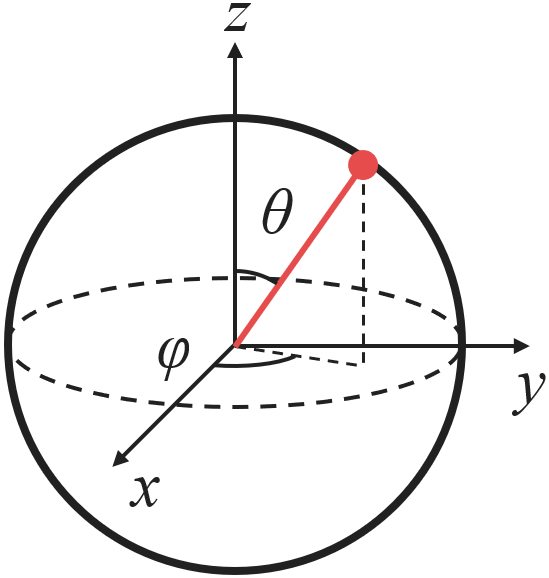
\includegraphics[width=0.35\columnwidth]{figures/bloch_sphere.png}
    \caption{ブロッホ球}
    \label{fig:chap1_bloch_shpere}
\end{figure}
この球のことをBloch球と呼び、
ブロッホ球内に示される位置ベクトルのことをBlochベクトルと呼ぶ(図\ref{fig:chap1_bloch_shpere})。
この表示により、0と1だけではなく、その重ね合わせ状態も取りうる量子ビットを幾何的にイメージすることが容易となる。

では古典ビットを並べることを量子ビットで行うとしたとき、
数式上ではどのようにあらわされるのか。
それはテンソル積\(\otimes\)と呼ばれるものを使って行う。
1番目の量子ビットが\(\ket{\psi}=a_0\ket{0}+a_1\ket{1}\)の状態、
2番目の量子ビットが\(\ket{\phi}=b_0\ket{0}+b_1\ket{1}\)の状態にあるとき
これらをまとめた系は
\begin{equation}\begin{aligned}[b]
    \ket{\psi}_1\otimes\ket{\phi}_2
    &=\qty(a_0\ket{0}_1+a_1\ket{1}_1)\otimes(b_0\ket{0}_2+b_1\ket{1}_2)\\
    &=a_0b_0\ket{0}_1\otimes\ket{0}_2+a_0b_1\ket{0}_1\otimes\ket{1}_2
        +a_1b_0\ket{1}_1\otimes\ket{0}_2+a_1b_1\ket{1}_1\otimes\ket{1}_2
\end{aligned}\end{equation}
のように表現される。
量子情報などの量子ビットが多数現れるような量子多体系においてはこのテンソル積を表す\(\otimes\)はしばし省略されて、
\begin{equation}\begin{aligned}[b]
    \ket{\psi}\ket{\phi}
    &=a_0b_0\ket{0}\ket{0}+a_0b_1\ket{0}\ket{1}
        +a_1b_0\ket{1}\ket{0}+a_1b_1\ket{1}\ket{1}\\
    &=a_0b_0\ket{00}+a_0b_1\ket{01}
        +a_1b_0\ket{10}+a_1b_1\ket{11}\label{eq:chap1_tensor_product_state}
\end{aligned}\end{equation}
のように書かれることも多い。

ここで特筆すべきこととして、1つの量子ビットを2つ持ってきてもすべての状態を表現できるわけではないことがある。
例えば
\begin{equation}\begin{aligned}[b]
    \ket{\psi} =\frac{1}{\sqrt{2}}\ket{00}+\frac{1}{\sqrt{2}}\ket{11}
    \label{eq:chap1_bell_state1}
\end{aligned}\end{equation}
という状態を考えてみる。
これが(\ref{eq:chap1_tensor_product_state})式で表せるとする。
\(\ket{01}\)の係数を両者で比較してみると\(a_0\)もしくは\(b_1\)のいずれかが0でなければならないことがわかる。
しかしそうしてしまうと、\(\ket{00}\)か\(\ket{11}\)のどちらかの係数が0になってしまい、本来の\(1/\sqrt{2}\)からずれてしまう。
これより矛盾であり、(\ref{eq:chap1_bell_state1})式のような状態はテンソル積で表すことはできないことが確認できた。
このような状態を量子もつれ状態(エンタングル状態)と呼ぶ。

なぜこれが量子もつれ状態と呼ばれるのか。
それは、この状態は2つの量子ビットが量子性によって非局所的につながった状態であるといえるからである。
例えば(\ref{eq:chap1_bell_state1})式の状態を考えてみる。
この状態は、1番目の量子ビットが\(\ket{0}\)のとき、2番目の量子ビットも\(\ket{0}\)であることを意味している。
同様に、1番目の量子ビットが\(\ket{1}\)のとき、2番目の量子ビットも\(\ket{1}\)であることを意味している。
これは1番目の量子ビットと2番目の量子ビットがどれだけ離れていても成り立つ性質である。
これはよくよく考えてみると非常に不思議である。
というのも、重ね合わせ状態にある1番目の量子ビットを観測して\(\ket{0}\)が得られたとすると状態は
\begin{equation}\begin{aligned}[b]
    \ket{\psi} = \frac{1}{\sqrt{2}}\ket{00}+\frac{1}{\sqrt{2}}\ket{11}
    \xrightarrow{\text{観測}} \ket{00}
\end{aligned}\end{equation}
のように即座に\(\ket{00}\)へと収縮してしまう。
つまり、1番目の量子ビットを測定したという情報が、光速でも伝わらないほど遠く離れていたとしても、
瞬時に2番目の量子ビットへと伝わったかのように状態も確定してしまうのである。
これは、情報が伝わる速度の上限は光速であるという相対性理論の原理に反して、
あたかも測定による影響が光速を超えて伝わったかのような振る舞いである。
このように、量子的な性質によって空間的に離れていても状態が非局所的に強く絡み合っていることから、
この状態は量子もつれと呼ばれるのである。

この量子もつれ状態は量子計算において重要な役割を果たす。
例えば、この量子もつれ状態を用いれば、人に知られたくない情報を第三者に漏れることなく伝えることができそうだなと気づくだろう。
これは実際、量子通信と呼ばれる分野で研究されている。
もちろん、本稿で扱う量子誤り訂正符号の構成においてもこの量子もつれ状態は重要な役割を果たすことになる。

\section{古典誤り訂正符号}
このセクションでは古典誤り訂正符号の基本的な性質や用語を説明する。
これらの性質や用語は量子誤り訂正符号にも共通のものが多く、
また、量子誤り訂正符号に比べシンプルなものであり、
量子誤り訂正符号を理解するための基礎となるものである。

情報を蓄えたり、伝達したりする媒体は常にノイズの影響を受ける。
これにより、古典ビットであらわされた情報の一部が誤ってしまうことがある。
最もシンプルなエラーは0と1が入れ替わってしまうような反転エラー(flip error)である。
このようなエラーから情報を守るために最も単純な方法は、同じ情報を複数回繰り返して保存することである。

例えばもともとの情報が 010 で表されてるとする。これを以下のように冗長化してみる。
\begin{equation}\begin{aligned}[b]
    010 \xrightarrow{\text{冗長化}} 000\,111\,000
\end{aligned}\end{equation}
すると、もしこのようにエラーが生じたとしても多数決によって単純に訂正することができる。
\begin{equation}\begin{aligned}[b]
    010
    \xrightarrow{\text{符号化}} 000\,111\,000
    \xrightarrow{\text{エラー}} 100\,101\,000
    \xrightarrow{\text{訂正}} 000\,111\,000
    \xrightarrow{\text{復号}} 010
\end{aligned}\end{equation}


\end{document}
